Having identified the various activities needed to be done, we now tried to make a plan, again, on how to reach the milestones in the project. This time around, we noticed that certain activities had dependencies between them i.e. the \textbf{EXAMPLE1} needed to be done before the \textbf{EXAMPLE2}.
We found it important to gain a firm understanding of the dependencies between our work activities, since we believed this would strengthen our ability to make a realistic plan. As such, we postponed the planning, and instead we strived to strengthen our understanding of the aforementioned dependencies. We decided to use a dependency diagram for this, more precisely a network diagram using the activity on-node format.
In this version of the network diagram, each box represents an activity with dependencies represented as arrows between them. The method uses the concepts of earliest start/finish times (EST/EFT) and latest start/finish times (LST/LFT) in addition to the activity’s own estimated duration.

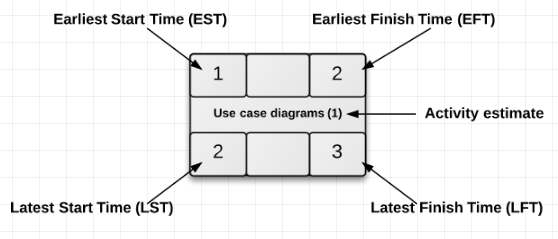
\includegraphics[scale=0.5]{./Empiri/Planning/img/networkdiagramnotation.png}
 
The EST/EFT can be found by a forward pass through the diagram, while the LST/LFTs can be found by a following backward pass.
These numbers introduce the concept of a critical path, which consists of those activities that, if delayed, would delay the whole project (in other words those that must keep the deadline). It also gives a clear presentation of the total slack (how much an activity can be postponed), free slack (how much an activity can be postponed without affecting following activities), and head slack (how much an activity can be postponed without delaying the whole project deadline) for each activity.
Our network diagram can be found in appendix \textbf{insert reference here}.